\documentclass{article}
\usepackage{amsmath}
\usepackage{amssymb}
\usepackage{graphicx}
\usepackage{hyperref}
\usepackage[version=4]{mhchem}


\begin{document}
\section*{Problem}
In any \(\triangle A B C, D, E\), and \(F\) are midpoints of the sides \(A C, A B\), and \(B C\), respectively. \(B G\) is an altitude of \(\triangle A B C\). Prove that \(\angle E G F\) \(=\angle E D F\).\\
\centering
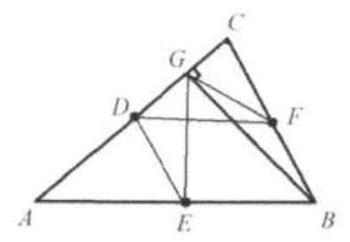
\includegraphics[width=\textwidth]{images/045.jpg}

\section*{Solution}
\begin{center}
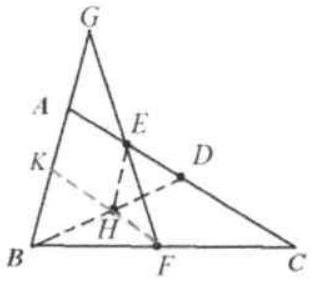
\includegraphics[width=\textwidth]{images/050.jpg}
\end{center}

Connect \(E F\). Since both \(E\) and \(F\) are midpoints of the sides \(A B\) and \(B C\), respectively, \(E F / / A C / / D G\).

Since \(D\) and \(E\) are midpoints of the sides \(A C\) and \(A B, D E\) is the midline of \(\triangle A B C\). Thus \(D E=C F\).

Since \(F G\) is the median of right \(\triangle B G C, G F=C F\).\\
So \(D E=G F\).\\
\centering
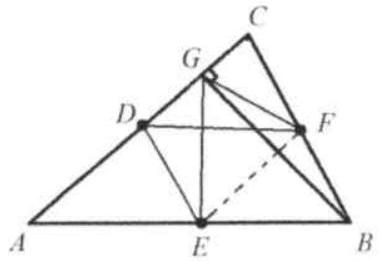
\includegraphics[width=\textwidth]{images/050(2).jpg}

Quadrilateral \(D G F E\) is an isosceles trapezoid.\\
Then \(\angle D E F=\angle D F E\).\\
Thus \(\triangle G F E \cong \triangle D E F(S A S)\), and \(\angle E G F=\angle E D F\).

\end{document}
